\section{Data Sources and Structure}
When we talk about any data, it is also necessary to take into consideration the data source. The same is true for urban data. A field of research called Urban Informatics focuses on the role of data generated in cities and urban environments.

\subsection{Urban Informatics}
In 2011, Forth et al. described Urban Informatics as a separate field of study. It focuses on three key aspects - place, technology, and people in the context of urban environments. The urban environment is described as a "complex techno-social network; the city only meaningfully exists when a sustained stream of people occupies it." The authors outline and study four dominant trends: the emergence of ubiquitous computing, the accessibility of real-time information, informed sustainability, and planning based on citizen participation. 

One of the goals of Urban Informatics is to help developing communication channels between local authorities and citizens. Moreover, thanks to the gathered information, the citizens can, directly and indirectly, influence the development of the urban area. The communication channels, as understood by Urban Informatics, are omnidirectional. The data is gathered and received through devices that are part of the ubicomp device system. Therefore, the ubicomp system can be understood as a data source. Additional data sources are local governments and online services, including social media. 

\paragraph{Ubicomp} Mark Weiser first introduced Ubiquitous Computing in 1991. The concept of ubicomp relies on small embedded computers, which communicate together and allow for seamless interaction between users and technology. On the level of cities, the ubiquitous information's impact became the focus of study in a field called Urban Computing. 

\paragraph{Participatory Sensing} In the spirit of ubiquitous computing, there is an emerging field of Participatory Sensing, which enables gathering data from devices of individual users. The design of the participation model focuses on data credibility, security, and privacy protection. One of the applications of Participatory Sensing is the use of the gathered data for urban planning. 

\paragraph{Open Data}
The most prominent source of data are governments and local institutions. The data is commonly released in several open formats, which are further described in a separate subsection. This data often includes maps, building layouts, terrain models, technical metadata, public transport data, etc. The formats range from generic CSV or SQLite-based to domain-specific DWG, CityGML, etc.   
The data presented earlier are mainly static; some cities also offer real-time information about weather or public transport vehicle locations. 

\paragraph{Online services}
Personal data can also be acquired from social networks or mobile phone carriers. Online platforms usually support geotagging, adding geospatial metadata to the content posted online. The content can be easily queried based on the selected location. Alternatively, the citizens' location can be tracked via their mobile phone directly by carriers using the individual base transceiver stations (BTS).  From the perspective of Urban Informatics, the aforementioned data sources enable creating richer urban area models. 

\subsection{Classes of Open Urban Data}
The following list has been aggregated based on open data available for the city of Prague. 

\begin{itemize}
    \item Buildings, Bridges, Spatial Features
    \item Terrain
    \item Flora
    \item City Structure Elements and Networks
    \item Public Service Buildings and Elements
    \item Public Transport + Trafic
    \item Noise Maps
    \item Weather + Air Quality
    \item Walkability
    \item Population density + movement
\end{itemize}

\begin{figure}[h]
    \centering
    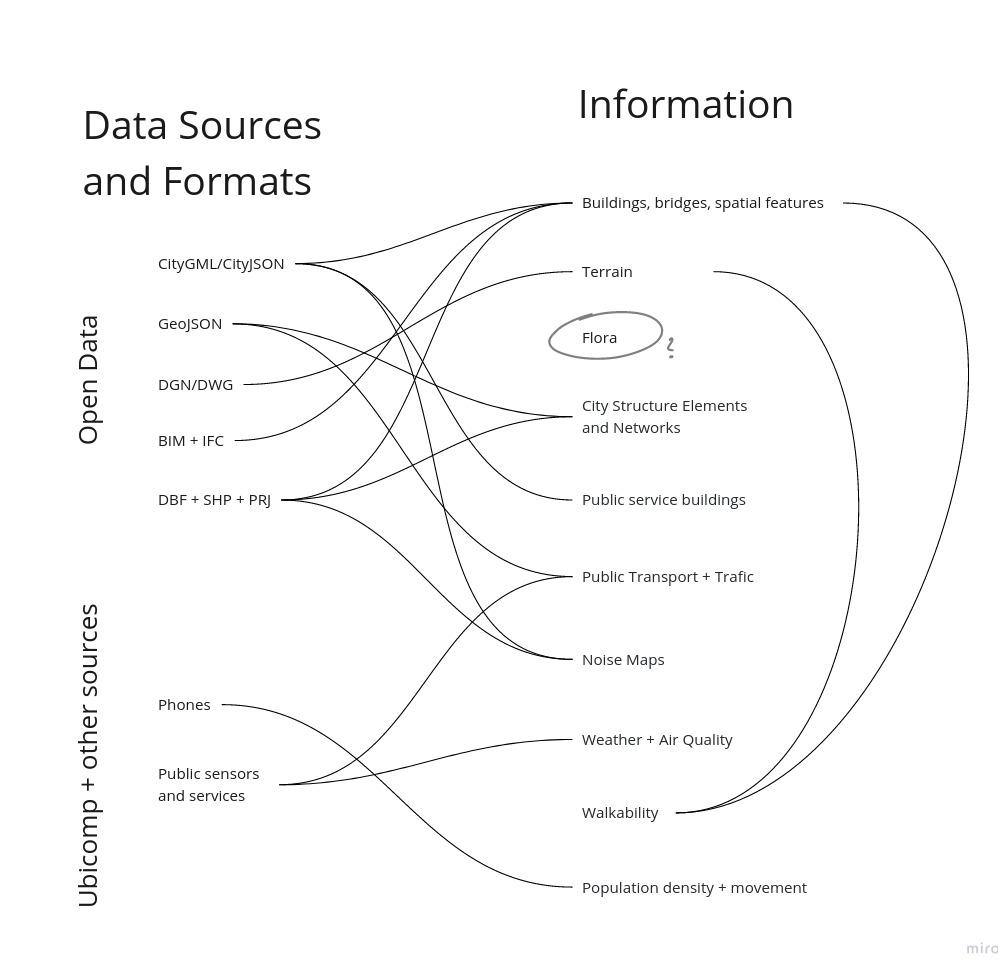
\includegraphics[width=\linewidth]{img/dataformats.jpg}
    \caption{Data sources and File Formats}
\end{figure}

There are several other important attributes, which are not freely available:
\begin{itemize}
    \item Land Price and Owners
    \item TODO
\end{itemize}

\subsection{File Formats}

The following list includes widely used file formats for urban data:

\paragraph{Esri Shapefiles} 
Shapefile is generally a vector data file format for a geographic information system. A list formats fall into the category of shapefiles, but the minimal set of files necessary for correct data interpretation is  DBF, SHP, and PRJ file. SHP contains the actual geometry, DBF contains the attributes and indexes, and the PRJ file describes the coordinate reference system. In the original specification, SHX is also a mandatory file. Still, the file only allows to accelerate the queries and is not required for the data to be displayed correctly. The Shapefile format is well documented, and there is a range of existing importers in various languages. 


\paragraph{CityGML and CityJSON}
CityGML is an XML-based file format designed to capture the structure and metadata of 3D city models. The aim of the development is to come up with a standardized and sustainable way of storing urban data. There is a JSON-based version of CityGML - CityJSON. Despite minor differences, these two standards are mostly compatible. From the practical point of view, the CityJSON format is much less verbose and thus easily parsable. Both CityGML and CityJSON are open formats, and there is a list of convertors and importers available.

\paragraph{GeoJSON}
Another JSON-based standard is the GeoJSON format. This GeoJSON structure is quite simple; the file can describe a set of primitive geometry objects such as lines, lines, or polygons. Each primitive can have a variable number of properties, which can be completely arbitrary. The GeoJSON file usually describes data such as networks or areas. Compared to CityJSON, GeoJSON is not suitable for representing hierarchies, which usually naturally appear in building geometry and its components. GeoJSON is an open format, it is fairly simple to write an importer for this format, and there are several available. 

\paragraph{DGN and DWG}
Both of these formats are proprietary vector formats used by CAD editors, such as AutoCAD. A reader for the DWG format is part of RealDWG developer suite created by Autodesk. Its license is incompatible with most free software licenses. As a result, no open tools contain an effective importer for the DWG file format. There is no official free DWG SDK; the software for importing and converting DWG is a part of software offered by OpenDesignAlliance (ODA). Some sort of DWG and DGN loading capabilities has the framework GDAL.

\paragraph{BIM and IFC}
BIM as the Building Information Model is the common name for all data relevant to an architectural structure - the plans, costs, changes over time, etc.  Industry Foundation Classes (IFC) is a data model designed for architectural, building, and construction data. It is a platform-neutral and open file format. In some states, the IFC has been legally established as the standard exchange format for public project data. Like Shapefiles, IFC is not a single file; there are many available IFC versions, and the development of newer ones is underway. On the other hand, contrary to Shapefiles, each IFC file version should include the same data; the only difference is in the encoding.
